\documentclass[a4paper]{book}
\usepackage{makeidx}
\usepackage{natbib}
\usepackage{graphicx}
\usepackage{multicol}
\usepackage{float}
\usepackage{listings}
\usepackage{color}
\usepackage{ifthen}
\usepackage[table]{xcolor}
\usepackage{textcomp}
\usepackage{alltt}
\usepackage{ifpdf}
\ifpdf
\usepackage[pdftex,
            pagebackref=true,
            colorlinks=true,
            linkcolor=blue,
            unicode
           ]{hyperref}
\else
\usepackage[ps2pdf,
            pagebackref=true,
            colorlinks=true,
            linkcolor=blue,
            unicode
           ]{hyperref}
\usepackage{pspicture}
\fi
\usepackage[utf8]{inputenc}
\usepackage{mathptmx}
\usepackage[scaled=.90]{helvet}
\usepackage{courier}
\usepackage{sectsty}
\usepackage[titles]{tocloft}
\usepackage{doxygen}
\lstset{language=C++,inputencoding=utf8,basicstyle=\footnotesize,breaklines=true,breakatwhitespace=true,tabsize=8,numbers=left }
\makeindex
\setcounter{tocdepth}{3}
\renewcommand{\footrulewidth}{0.4pt}
\renewcommand{\familydefault}{\sfdefault}
\hfuzz=15pt
\setlength{\emergencystretch}{15pt}
\hbadness=750
\tolerance=750
\begin{document}
\hypersetup{pageanchor=false,citecolor=blue}
\begin{titlepage}
\vspace*{7cm}
\begin{center}
{\Large \-Lab 11 -\/ \-Heap \-Implementation }\\
\vspace*{1cm}
{\large \-Generated by Doxygen 1.7.6.1}\\
\vspace*{0.5cm}
{\small Wed Nov 13 2013 17:55:18}\\
\end{center}
\end{titlepage}
\clearemptydoublepage
\pagenumbering{roman}
\tableofcontents
\clearemptydoublepage
\pagenumbering{arabic}
\hypersetup{pageanchor=true,citecolor=blue}
\chapter{\-Class \-Index}
\section{\-Class \-Hierarchy}
\-This inheritance list is sorted roughly, but not completely, alphabetically\-:\begin{DoxyCompactList}
\item \contentsline{section}{\-Greater$<$ \-Key\-Type $>$}{\pageref{class_greater}}{}
\item \contentsline{section}{\-Heap$<$ \-Data\-Type, \-Key\-Type, \-Comparator $>$}{\pageref{class_heap}}{}
\item \contentsline{section}{\-Heap$<$ \-Data\-Type $>$}{\pageref{class_heap}}{}
\begin{DoxyCompactList}
\item \contentsline{section}{\-Priority\-Queue$<$ \-Data\-Type, \-Key\-Type, \-Comparator $>$}{\pageref{class_priority_queue}}{}
\end{DoxyCompactList}
\item \contentsline{section}{\-Less$<$ \-Key\-Type $>$}{\pageref{class_less}}{}
\item \contentsline{section}{\-Less$<$ int $>$}{\pageref{class_less}}{}
\item \contentsline{section}{\-Task\-Data}{\pageref{struct_task_data}}{}
\item \contentsline{section}{\-Test\-Data}{\pageref{class_test_data}}{}
\item \contentsline{section}{\-Test\-Data\-Item$<$ \-Key\-Type $>$}{\pageref{class_test_data_item}}{}
\end{DoxyCompactList}

\chapter{\-Class \-Index}
\section{\-Class \-List}
\-Here are the classes, structs, unions and interfaces with brief descriptions\-:\begin{DoxyCompactList}
\item\contentsline{section}{\hyperlink{struct_account_record}{\-Account\-Record} }{\pageref{struct_account_record}}{}
\item\contentsline{section}{\hyperlink{class_b_s_tree}{\-B\-S\-Tree$<$ Data\-Type, Key\-Type $>$} }{\pageref{class_b_s_tree}}{}
\item\contentsline{section}{\hyperlink{class_b_s_tree_1_1_b_s_tree_node}{\-B\-S\-Tree$<$ Data\-Type, Key\-Type $>$\-::\-B\-S\-Tree\-Node} }{\pageref{class_b_s_tree_1_1_b_s_tree_node}}{}
\item\contentsline{section}{\hyperlink{struct_index_entry}{\-Index\-Entry} }{\pageref{struct_index_entry}}{}
\item\contentsline{section}{\hyperlink{class_test_data}{\-Test\-Data} }{\pageref{class_test_data}}{}
\end{DoxyCompactList}

\chapter{\-File \-Index}
\section{\-File \-List}
\-Here is a list of all files with brief descriptions\-:\begin{DoxyCompactList}
\item\contentsline{section}{\hyperlink{_b_s_tree_8cpp}{\-B\-S\-Tree.\-cpp} }{\pageref{_b_s_tree_8cpp}}{}
\item\contentsline{section}{\hyperlink{_b_s_tree_8h}{\-B\-S\-Tree.\-h} }{\pageref{_b_s_tree_8h}}{}
\item\contentsline{section}{\hyperlink{config_8h}{config.\-h} }{\pageref{config_8h}}{}
\item\contentsline{section}{\hyperlink{database_8cpp}{database.\-cpp} }{\pageref{database_8cpp}}{}
\item\contentsline{section}{\hyperlink{show9_8cpp}{show9.\-cpp} }{\pageref{show9_8cpp}}{}
\item\contentsline{section}{\hyperlink{test9_8cpp}{test9.\-cpp} }{\pageref{test9_8cpp}}{}
\end{DoxyCompactList}

\chapter{\-Class \-Documentation}
\hypertarget{class_greater}{\section{\-Greater$<$ \-Key\-Type $>$ \-Class \-Template \-Reference}
\label{class_greater}\index{\-Greater$<$ Key\-Type $>$@{\-Greater$<$ Key\-Type $>$}}
}
\subsection*{\-Public \-Member \-Functions}
\begin{DoxyCompactItemize}
\item 
bool \hyperlink{class_greater_a79d9cb7121723ee9d65b11cb2fce0379}{operator()} (const \-Key\-Type \&a, const \-Key\-Type \&b) const 
\end{DoxyCompactItemize}
\subsubsection*{template$<$typename Key\-Type = int$>$ class Greater$<$ Key\-Type $>$}



\subsection{\-Member \-Function \-Documentation}
\hypertarget{class_greater_a79d9cb7121723ee9d65b11cb2fce0379}{\index{\-Greater@{\-Greater}!operator()@{operator()}}
\index{operator()@{operator()}!Greater@{\-Greater}}
\subsubsection[{operator()}]{\setlength{\rightskip}{0pt plus 5cm}template$<$typename Key\-Type  = int$>$ bool {\bf \-Greater}$<$ \-Key\-Type $>$\-::operator() (
\begin{DoxyParamCaption}
\item[{const \-Key\-Type \&}]{a, }
\item[{const \-Key\-Type \&}]{b}
\end{DoxyParamCaption}
) const\hspace{0.3cm}{\ttfamily  \mbox{[}inline\mbox{]}}}}\label{class_greater_a79d9cb7121723ee9d65b11cb2fce0379}


\-The documentation for this class was generated from the following file\-:\begin{DoxyCompactItemize}
\item 
\hyperlink{test11_8cpp}{test11.\-cpp}\end{DoxyCompactItemize}

\hypertarget{class_heap}{\section{\-Heap$<$ \-Data\-Type, \-Key\-Type, \-Comparator $>$ \-Class \-Template \-Reference}
\label{class_heap}\index{\-Heap$<$ Data\-Type, Key\-Type, Comparator $>$@{\-Heap$<$ Data\-Type, Key\-Type, Comparator $>$}}
}


{\ttfamily \#include $<$\-Heap.\-h$>$}

\subsection*{\-Public \-Member \-Functions}
\begin{DoxyCompactItemize}
\item 
\hyperlink{class_heap_ae17e34e3c86d88263a8fdf80b9ba78fc}{\-Heap} (int max\-Number=\hyperlink{class_heap_a967c19732a20a72e8e824402ad6763c8}{\-D\-E\-F\-A\-U\-L\-T\-\_\-\-M\-A\-X\-\_\-\-H\-E\-A\-P\-\_\-\-S\-I\-Z\-E})
\item 
\hyperlink{class_heap_a97e3b462be1c6af31d7519546bba8907}{\-Heap} (const \hyperlink{class_heap}{\-Heap} \&other)
\item 
\hyperlink{class_heap}{\-Heap} \& \hyperlink{class_heap_a5ed119341c39bcea1437321d4247dd40}{operator=} (const \hyperlink{class_heap}{\-Heap} \&other)
\item 
\hyperlink{class_heap_a555ade7891007de959bef0ee53e28767}{$\sim$\-Heap} ()
\item 
void \hyperlink{class_heap_aa68cf80454ab1b246fa723612805a91e}{insert} (const \-Data\-Type \&new\-Data\-Item)  throw ( logic\-\_\-error )
\item 
\-Data\-Type \hyperlink{class_heap_a4a18bfdacd897c45fc3da13f22b8930d}{remove} ()  throw ( logic\-\_\-error )
\item 
void \hyperlink{class_heap_a19a78c8eae2cf7c8253e34e54d86ed73}{clear} ()
\item 
bool \hyperlink{class_heap_ab8fa26d416ac0e27dfcbf18c54f8f73f}{is\-Empty} () const 
\item 
bool \hyperlink{class_heap_ac9111b884c74a376240e0155a788756e}{is\-Full} () const 
\item 
void \hyperlink{class_heap_a3ae1e1f27a145749c8b9f2da777cb8bc}{show\-Structure} () const 
\item 
void \hyperlink{class_heap_a4bdb1772ea92899de245d6cbd217d085}{write\-Levels} () const 
\end{DoxyCompactItemize}
\subsection*{\-Static \-Public \-Attributes}
\begin{DoxyCompactItemize}
\item 
static const int \hyperlink{class_heap_a967c19732a20a72e8e824402ad6763c8}{\-D\-E\-F\-A\-U\-L\-T\-\_\-\-M\-A\-X\-\_\-\-H\-E\-A\-P\-\_\-\-S\-I\-Z\-E} = 10
\end{DoxyCompactItemize}
\subsection*{\-Private \-Member \-Functions}
\begin{DoxyCompactItemize}
\item 
void \hyperlink{class_heap_a49a54dd4782e6c68f14a5df3ba4da7af}{show\-Subtree} (int index, int level) const 
\item 
int \hyperlink{class_heap_a039940a2aa70c00997e1f3285f90a9d1}{parent} (int c\-Index) const 
\item 
int \hyperlink{class_heap_a80ec118ed1d98113a3b6765a98d8ef30}{lchild} (int p\-Index) const 
\item 
int \hyperlink{class_heap_a25b1ff34ed504c8bdb81cbadd8c7ad3d}{rchild} (int p\-Index) const 
\end{DoxyCompactItemize}
\subsection*{\-Private \-Attributes}
\begin{DoxyCompactItemize}
\item 
int \hyperlink{class_heap_a7f8e5c3cc64b8799b4e75b5a0f675e69}{max\-Size}
\item 
int \hyperlink{class_heap_a0964c2d309605bee2f6f1a9cee9ab89a}{size}
\item 
\-Data\-Type $\ast$ \hyperlink{class_heap_ace779ec73409a031eda4a7c1b898eb56}{data\-Items}
\item 
\-Comparator \hyperlink{class_heap_adc20ebd4d97dff37f19ced91ccdc4560}{comparator}
\end{DoxyCompactItemize}
\subsubsection*{template$<$typename \-Data\-Type, typename \-Key\-Type = int, typename \-Comparator = \-Less$<$\-Key\-Type$>$$>$ class Heap$<$ Data\-Type, Key\-Type, Comparator $>$}



\subsection{\-Constructor \& \-Destructor \-Documentation}
\hypertarget{class_heap_ae17e34e3c86d88263a8fdf80b9ba78fc}{\index{\-Heap@{\-Heap}!\-Heap@{\-Heap}}
\index{\-Heap@{\-Heap}!Heap@{\-Heap}}
\subsubsection[{\-Heap}]{\setlength{\rightskip}{0pt plus 5cm}template$<$typename Data\-Type , typename Key\-Type , typename Comparator $>$ {\bf \-Heap}$<$ \-Data\-Type, \-Key\-Type, \-Comparator $>$\-::{\bf \-Heap} (
\begin{DoxyParamCaption}
\item[{int}]{max\-Number = {\ttfamily {\bf \-D\-E\-F\-A\-U\-L\-T\-\_\-\-M\-A\-X\-\_\-\-H\-E\-A\-P\-\_\-\-S\-I\-Z\-E}}}
\end{DoxyParamCaption}
)}}\label{class_heap_ae17e34e3c86d88263a8fdf80b9ba78fc}
\-Default \-Constructor

\-Default constructor which creats an empty heap. \-Allocates memory for heap of given size.

{\bfseries \-Algorithm} 
\begin{DoxyEnumerate}
\item \-Set max\-Size equal to max\-Number.
\item \-Set size to 0 to designate empty heap.
\item \-Allocate array of size max\-Size and assign data\-Items to point to this array.
\end{DoxyEnumerate}

\begin{DoxyPrecond}{\-Precondition}

\begin{DoxyEnumerate}
\item \-Function must be called with valid integer for max\-Number.
\end{DoxyEnumerate}
\end{DoxyPrecond}
\begin{DoxyPostcond}{\-Postcondition}

\begin{DoxyEnumerate}
\item \-All data members will be updated.
\item data\-Items will now have memory allocated to it.
\end{DoxyEnumerate}
\end{DoxyPostcond}

\begin{DoxyParams}{\-Parameters}
{\em max\-Number} & \-Integer variable designating size of heap. \-This integer has a default value of \-Default\-\_\-\-Max\-\_\-\-Heap\-\_\-\-Size = 10.\\
\hline
\end{DoxyParams}
\begin{DoxyReturn}{\-Returns}
\-None
\end{DoxyReturn}

\begin{DoxyExceptions}{\-Exceptions}
{\em } & \\
\hline
\end{DoxyExceptions}
\hypertarget{class_heap_a97e3b462be1c6af31d7519546bba8907}{\index{\-Heap@{\-Heap}!\-Heap@{\-Heap}}
\index{\-Heap@{\-Heap}!Heap@{\-Heap}}
\subsubsection[{\-Heap}]{\setlength{\rightskip}{0pt plus 5cm}template$<$typename Data\-Type , typename Key\-Type , typename Comparator $>$ {\bf \-Heap}$<$ \-Data\-Type, \-Key\-Type, \-Comparator $>$\-::{\bf \-Heap} (
\begin{DoxyParamCaption}
\item[{const {\bf \-Heap}$<$ \-Data\-Type, \-Key\-Type, \-Comparator $>$ \&}]{other}
\end{DoxyParamCaption}
)}}\label{class_heap_a97e3b462be1c6af31d7519546bba8907}
\-Copy \-Constructor

\-Copy constructor initializes a heap which will be set to a deep copy of the given heap from the parameter.

{\bfseries \-Algorithm} 
\begin{DoxyEnumerate}
\item \-Set all data members equal to equivalent data members of other heap.
\item \-Allocate memory for data\-Items of array of \-Data\-Type with size max\-Size.
\item \-Assign current heap to other heap.
\end{DoxyEnumerate}

\begin{DoxyPrecond}{\-Precondition}

\begin{DoxyEnumerate}
\item \-Function must be called with valid heap as parameter.
\end{DoxyEnumerate}
\end{DoxyPrecond}
\begin{DoxyPostcond}{\-Postcondition}

\begin{DoxyEnumerate}
\item \-All data members of current heap will be updated.
\item data\-Items will have memory allocated to it.
\item \-Contents of data\-Items will be equivalent to dataitems of other heap.
\end{DoxyEnumerate}
\end{DoxyPostcond}

\begin{DoxyParams}{\-Parameters}
{\em other} & \hyperlink{class_heap}{\-Heap} object to be copied to current heap.\\
\hline
\end{DoxyParams}
\begin{DoxyReturn}{\-Returns}
\-None
\end{DoxyReturn}

\begin{DoxyExceptions}{\-Exceptions}
{\em } & \\
\hline
\end{DoxyExceptions}
\hypertarget{class_heap_a555ade7891007de959bef0ee53e28767}{\index{\-Heap@{\-Heap}!$\sim$\-Heap@{$\sim$\-Heap}}
\index{$\sim$\-Heap@{$\sim$\-Heap}!Heap@{\-Heap}}
\subsubsection[{$\sim$\-Heap}]{\setlength{\rightskip}{0pt plus 5cm}template$<$typename Data\-Type , typename Key\-Type , typename Comparator $>$ {\bf \-Heap}$<$ \-Data\-Type, \-Key\-Type, \-Comparator $>$\-::$\sim${\bf \-Heap} (
\begin{DoxyParamCaption}
{}
\end{DoxyParamCaption}
)}}\label{class_heap_a555ade7891007de959bef0ee53e28767}
\-Destructor

\-Deallocates the memory used to store the heap. \-Resets other data members to indicate an empty heap.

{\bfseries \-Algorithm} 
\begin{DoxyEnumerate}
\item \-If data\-Items has memory allocated to it, deallocate this memory.
\item \-Set max\-Size and actual size to zero.
\end{DoxyEnumerate}

\begin{DoxyPrecond}{\-Precondition}

\begin{DoxyEnumerate}
\item \hyperlink{class_heap}{\-Heap} must be initialized and should have memory allocated to it.
\end{DoxyEnumerate}
\end{DoxyPrecond}
\begin{DoxyPostcond}{\-Postcondition}

\begin{DoxyEnumerate}
\item \hyperlink{class_heap}{\-Heap} will no longer have memory allocated to it.
\item \-Data members will be updated to indicate empty heap.
\end{DoxyEnumerate}
\end{DoxyPostcond}

\begin{DoxyParams}{\-Parameters}
{\em \-None} & \\
\hline
\end{DoxyParams}
\begin{DoxyReturn}{\-Returns}
\-None
\end{DoxyReturn}

\begin{DoxyExceptions}{\-Exceptions}
{\em } & \\
\hline
\end{DoxyExceptions}


\subsection{\-Member \-Function \-Documentation}
\hypertarget{class_heap_a19a78c8eae2cf7c8253e34e54d86ed73}{\index{\-Heap@{\-Heap}!clear@{clear}}
\index{clear@{clear}!Heap@{\-Heap}}
\subsubsection[{clear}]{\setlength{\rightskip}{0pt plus 5cm}template$<$typename Data\-Type , typename Key\-Type , typename Comparator $>$ void {\bf \-Heap}$<$ \-Data\-Type, \-Key\-Type, \-Comparator $>$\-::{\bf clear} (
\begin{DoxyParamCaption}
{}
\end{DoxyParamCaption}
)}}\label{class_heap_a19a78c8eae2cf7c8253e34e54d86ed73}
\-Clear

\-Removes all data items from the heap.

{\bfseries \-Algorithm} 
\begin{DoxyEnumerate}
\item \-Set number of actual data items to zero.
\end{DoxyEnumerate}

\begin{DoxyPrecond}{\-Precondition}

\begin{DoxyEnumerate}
\item \hyperlink{class_heap}{\-Heap} must be declared and have memory allocated to it.
\end{DoxyEnumerate}
\end{DoxyPrecond}
\begin{DoxyPostcond}{\-Postcondition}

\begin{DoxyEnumerate}
\item \-Number of actual items will be set to 0.
\end{DoxyEnumerate}
\end{DoxyPostcond}

\begin{DoxyParams}{\-Parameters}
{\em \-None} & \\
\hline
\end{DoxyParams}
\begin{DoxyReturn}{\-Returns}
\-None
\end{DoxyReturn}

\begin{DoxyExceptions}{\-Exceptions}
{\em \-None} & \\
\hline
\end{DoxyExceptions}
\hypertarget{class_heap_aa68cf80454ab1b246fa723612805a91e}{\index{\-Heap@{\-Heap}!insert@{insert}}
\index{insert@{insert}!Heap@{\-Heap}}
\subsubsection[{insert}]{\setlength{\rightskip}{0pt plus 5cm}template$<$typename \-Data\-Type, typename Key\-Type , typename Comparator $>$ void {\bf \-Heap}$<$ \-Data\-Type, \-Key\-Type, \-Comparator $>$\-::{\bf insert} (
\begin{DoxyParamCaption}
\item[{const \-Data\-Type \&}]{new\-Data\-Item}
\end{DoxyParamCaption}
)  throw ( logic\-\_\-error )}}\label{class_heap_aa68cf80454ab1b246fa723612805a91e}
\-Insert

\-Description

{\bfseries \-Algorithm} 
\begin{DoxyEnumerate}
\item 
\item 
\end{DoxyEnumerate}

\begin{DoxyPrecond}{\-Precondition}

\begin{DoxyEnumerate}
\item 
\item 
\end{DoxyEnumerate}
\end{DoxyPrecond}
\begin{DoxyPostcond}{\-Postcondition}

\begin{DoxyEnumerate}
\item 
\item 
\end{DoxyEnumerate}
\end{DoxyPostcond}

\begin{DoxyParams}{\-Parameters}
{\em \-None} & \\
\hline
\end{DoxyParams}
\begin{DoxyReturn}{\-Returns}
\-None
\end{DoxyReturn}

\begin{DoxyExceptions}{\-Exceptions}
{\em } & \\
\hline
\end{DoxyExceptions}
\hypertarget{class_heap_ab8fa26d416ac0e27dfcbf18c54f8f73f}{\index{\-Heap@{\-Heap}!is\-Empty@{is\-Empty}}
\index{is\-Empty@{is\-Empty}!Heap@{\-Heap}}
\subsubsection[{is\-Empty}]{\setlength{\rightskip}{0pt plus 5cm}template$<$typename Data\-Type , typename Key\-Type , typename Comparator $>$ bool {\bf \-Heap}$<$ \-Data\-Type, \-Key\-Type, \-Comparator $>$\-::{\bf is\-Empty} (
\begin{DoxyParamCaption}
{}
\end{DoxyParamCaption}
) const}}\label{class_heap_ab8fa26d416ac0e27dfcbf18c54f8f73f}
\-Is\-Empty

\-Function determines whether heap is empty. \-Returns true if heap is empty.

{\bfseries \-Algorithm} 
\begin{DoxyEnumerate}
\item \-Determine whether actual size is equal to zero.
\item \-Returns true if it is.
\end{DoxyEnumerate}

\begin{DoxyPrecond}{\-Precondition}

\begin{DoxyEnumerate}
\item \hyperlink{class_heap}{\-Heap} must be initialized.
\end{DoxyEnumerate}
\end{DoxyPrecond}
\begin{DoxyPostcond}{\-Postcondition}

\begin{DoxyEnumerate}
\item \hyperlink{class_heap}{\-Heap} will be unchanged.
\end{DoxyEnumerate}
\end{DoxyPostcond}

\begin{DoxyParams}{\-Parameters}
{\em \-None} & \\
\hline
\end{DoxyParams}
\begin{DoxyReturn}{\-Returns}
\-Boolean value. \-Returns true is heap is empty. \-Otherwise, returns false.
\end{DoxyReturn}

\begin{DoxyExceptions}{\-Exceptions}
{\em \-None} & \\
\hline
\end{DoxyExceptions}
\hypertarget{class_heap_ac9111b884c74a376240e0155a788756e}{\index{\-Heap@{\-Heap}!is\-Full@{is\-Full}}
\index{is\-Full@{is\-Full}!Heap@{\-Heap}}
\subsubsection[{is\-Full}]{\setlength{\rightskip}{0pt plus 5cm}template$<$typename Data\-Type , typename Key\-Type , typename Comparator $>$ bool {\bf \-Heap}$<$ \-Data\-Type, \-Key\-Type, \-Comparator $>$\-::{\bf is\-Full} (
\begin{DoxyParamCaption}
{}
\end{DoxyParamCaption}
) const}}\label{class_heap_ac9111b884c74a376240e0155a788756e}
\-Is\-Full

\-Function determines whether heap is full. \-Returns true if heap is full.

{\bfseries \-Algorithm} 
\begin{DoxyEnumerate}
\item \-Determine whether actual size is equal to max\-Size.
\item \-Returns true if it is.
\end{DoxyEnumerate}

\begin{DoxyPrecond}{\-Precondition}

\begin{DoxyEnumerate}
\item \hyperlink{class_heap}{\-Heap} must be initialized.
\end{DoxyEnumerate}
\end{DoxyPrecond}
\begin{DoxyPostcond}{\-Postcondition}

\begin{DoxyEnumerate}
\item \hyperlink{class_heap}{\-Heap} will be unchanged.
\end{DoxyEnumerate}
\end{DoxyPostcond}

\begin{DoxyParams}{\-Parameters}
{\em \-None} & \\
\hline
\end{DoxyParams}
\begin{DoxyReturn}{\-Returns}
\-Boolean value. \-Returns true is heap is full. \-Otherwise, returns false.
\end{DoxyReturn}

\begin{DoxyExceptions}{\-Exceptions}
{\em \-None} & \\
\hline
\end{DoxyExceptions}
\hypertarget{class_heap_a80ec118ed1d98113a3b6765a98d8ef30}{\index{\-Heap@{\-Heap}!lchild@{lchild}}
\index{lchild@{lchild}!Heap@{\-Heap}}
\subsubsection[{lchild}]{\setlength{\rightskip}{0pt plus 5cm}template$<$typename Data\-Type , typename Key\-Type , typename Comparator $>$ int {\bf \-Heap}$<$ \-Data\-Type, \-Key\-Type, \-Comparator $>$\-::{\bf lchild} (
\begin{DoxyParamCaption}
\item[{int}]{p\-Index}
\end{DoxyParamCaption}
) const\hspace{0.3cm}{\ttfamily  \mbox{[}private\mbox{]}}}}\label{class_heap_a80ec118ed1d98113a3b6765a98d8ef30}
lchild

\-Function calculates and returns the index of the left child of the given index, if index is valid. \-This assumes that any error checking for out of bounds is handled outside of the function.

{\bfseries \-Algorithm} 
\begin{DoxyEnumerate}
\item \-If index is valid (greater than or equal to zero), calculate left child index. \-This index is twice the parent index plus one.
\item \-Otherwise, set the left child index equal to negative one to designate an out of bounds index.
\item \-Return left child index.
\end{DoxyEnumerate}

\begin{DoxyPrecond}{\-Precondition}

\begin{DoxyEnumerate}
\item \-Function must be called with valid integer for parameter. \-This parameter does not have to be within bounds of the array, but should be.
\end{DoxyEnumerate}
\end{DoxyPrecond}
\begin{DoxyPostcond}{\-Postcondition}

\begin{DoxyEnumerate}
\item \-The heap will be unchanged.
\item \-The calculated value will be returned to the calling function.
\end{DoxyEnumerate}
\end{DoxyPostcond}

\begin{DoxyParams}{\-Parameters}
{\em p\-Index} & \-Integer value indicating the index of the parent item which is used to calculate the left child index.\\
\hline
\end{DoxyParams}
\begin{DoxyReturn}{\-Returns}
\-Integer value of the index of the right child, if it exists. \-Otherwise, negative one.
\end{DoxyReturn}

\begin{DoxyExceptions}{\-Exceptions}
{\em \-None} & \\
\hline
\end{DoxyExceptions}
\hypertarget{class_heap_a5ed119341c39bcea1437321d4247dd40}{\index{\-Heap@{\-Heap}!operator=@{operator=}}
\index{operator=@{operator=}!Heap@{\-Heap}}
\subsubsection[{operator=}]{\setlength{\rightskip}{0pt plus 5cm}template$<$typename Data\-Type , typename Key\-Type , typename Comparator $>$ {\bf \-Heap}$<$ \-Data\-Type, \-Key\-Type, \-Comparator $>$ \& {\bf \-Heap}$<$ \-Data\-Type, \-Key\-Type, \-Comparator $>$\-::operator= (
\begin{DoxyParamCaption}
\item[{const {\bf \-Heap}$<$ \-Data\-Type, \-Key\-Type, \-Comparator $>$ \&}]{other}
\end{DoxyParamCaption}
)}}\label{class_heap_a5ed119341c39bcea1437321d4247dd40}
\-Overloaded assignment operator

\-Overloaded assignment operator which sets the current heap to be a deep copy of the other heap. \-Returns current heap object.

{\bfseries \-Algorithm} 
\begin{DoxyEnumerate}
\item \-Check if current object has the same address of other heap.
\item \-If not, check if max\-Size of current heap is different from other max\-Size.
\item \-If it is, then set max\-Size equal to max\-Size of other heap.
\item \-Deallocate memory allocated to data\-Items.
\item \-Reallocate memory of new size.
\item \-Set actual size equal to actual size of other heap.
\item \-Iterate through other heap and copy contents to current heap.
\item \-Return current heap.
\end{DoxyEnumerate}

\begin{DoxyPrecond}{\-Precondition}

\begin{DoxyEnumerate}
\item \-Function must be called with valid heap object as parameter.
\item \-Other heap object must be previously initialized and have memory allocated to it.
\item \-Current heap object must be previously initialized and have memory allocated to it.
\end{DoxyEnumerate}
\end{DoxyPrecond}
\begin{DoxyPostcond}{\-Postcondition}

\begin{DoxyEnumerate}
\item \-Current heap will be updated to be a deep copy of other heap.
\item \-Other heap will be unchanged.
\end{DoxyEnumerate}
\end{DoxyPostcond}

\begin{DoxyParams}{\-Parameters}
{\em other} & \hyperlink{class_heap}{\-Heap} object to be copied to current heap.\\
\hline
\end{DoxyParams}
\begin{DoxyReturn}{\-Returns}
\hyperlink{class_heap}{\-Heap} object of current heap.
\end{DoxyReturn}

\begin{DoxyExceptions}{\-Exceptions}
{\em } & \\
\hline
\end{DoxyExceptions}
\hypertarget{class_heap_a039940a2aa70c00997e1f3285f90a9d1}{\index{\-Heap@{\-Heap}!parent@{parent}}
\index{parent@{parent}!Heap@{\-Heap}}
\subsubsection[{parent}]{\setlength{\rightskip}{0pt plus 5cm}template$<$typename Data\-Type , typename Key\-Type , typename Comparator $>$ int {\bf \-Heap}$<$ \-Data\-Type, \-Key\-Type, \-Comparator $>$\-::{\bf parent} (
\begin{DoxyParamCaption}
\item[{int}]{c\-Index}
\end{DoxyParamCaption}
) const\hspace{0.3cm}{\ttfamily  \mbox{[}private\mbox{]}}}}\label{class_heap_a039940a2aa70c00997e1f3285f90a9d1}
\-Parent

\-Function calculates and returns the index of the parent of the given index, if index is valid. \-This assumes that any error checking for out of bounds is handled outside of the function.

{\bfseries \-Algorithm} 
\begin{DoxyEnumerate}
\item \-If index is valid (greater than or equal to zero and within array), calculate parent index. \-This index is the child index minus one, all divided by two.
\item \-Otherwise, set the parent index equal to negative one to designate an out of bounds index.
\item \-Return parent index.
\end{DoxyEnumerate}

\begin{DoxyPrecond}{\-Precondition}

\begin{DoxyEnumerate}
\item \-Function must be called with valid integer for parameter. \-This parameter does not have to be within bounds of the array, but should be.
\end{DoxyEnumerate}
\end{DoxyPrecond}
\begin{DoxyPostcond}{\-Postcondition}

\begin{DoxyEnumerate}
\item \-The heap will be unchanged.
\item \-The calculated value will be returned to the calling function.
\end{DoxyEnumerate}
\end{DoxyPostcond}

\begin{DoxyParams}{\-Parameters}
{\em p\-Index} & \-Integer value indicating the index of the child item which is used to calculate the parent index.\\
\hline
\end{DoxyParams}
\begin{DoxyReturn}{\-Returns}
\-Integer value of the index of the parent, if it exists. \-Otherwise, negative one.
\end{DoxyReturn}

\begin{DoxyExceptions}{\-Exceptions}
{\em \-None} & \\
\hline
\end{DoxyExceptions}
\hypertarget{class_heap_a25b1ff34ed504c8bdb81cbadd8c7ad3d}{\index{\-Heap@{\-Heap}!rchild@{rchild}}
\index{rchild@{rchild}!Heap@{\-Heap}}
\subsubsection[{rchild}]{\setlength{\rightskip}{0pt plus 5cm}template$<$typename Data\-Type , typename Key\-Type , typename Comparator $>$ int {\bf \-Heap}$<$ \-Data\-Type, \-Key\-Type, \-Comparator $>$\-::{\bf rchild} (
\begin{DoxyParamCaption}
\item[{int}]{p\-Index}
\end{DoxyParamCaption}
) const\hspace{0.3cm}{\ttfamily  \mbox{[}private\mbox{]}}}}\label{class_heap_a25b1ff34ed504c8bdb81cbadd8c7ad3d}
rchild

\-Function calculates and returns the index of the right child of the given index, if index is valid. \-This assumes that any error checking for out of bounds is handled outside of the function.

{\bfseries \-Algorithm} 
\begin{DoxyEnumerate}
\item \-If index is valid (greater than or equal to zero), calculate right child index. \-This index is twice the parent index plus two.
\item \-Otherwise, set the right child index equal to negative one to designate an out of bounds index.
\item \-Return right child index.
\end{DoxyEnumerate}

\begin{DoxyPrecond}{\-Precondition}

\begin{DoxyEnumerate}
\item \-Function must be called with valid integer for parameter. \-This parameter does not have to be within bounds of the array, but should be.
\end{DoxyEnumerate}
\end{DoxyPrecond}
\begin{DoxyPostcond}{\-Postcondition}

\begin{DoxyEnumerate}
\item \-The heap will be unchanged.
\item \-The calculated value will be returned to the calling function.
\end{DoxyEnumerate}
\end{DoxyPostcond}

\begin{DoxyParams}{\-Parameters}
{\em p\-Index} & \-Integer value indicating the index of the parent item which is used to calculate the right child index.\\
\hline
\end{DoxyParams}
\begin{DoxyReturn}{\-Returns}
\-Integer value of the index of the right child, if it exists. \-Otherwise, negative one.
\end{DoxyReturn}

\begin{DoxyExceptions}{\-Exceptions}
{\em \-None} & \\
\hline
\end{DoxyExceptions}
\hypertarget{class_heap_a4a18bfdacd897c45fc3da13f22b8930d}{\index{\-Heap@{\-Heap}!remove@{remove}}
\index{remove@{remove}!Heap@{\-Heap}}
\subsubsection[{remove}]{\setlength{\rightskip}{0pt plus 5cm}template$<$typename Data\-Type , typename Key\-Type , typename Comparator $>$ \-Data\-Type {\bf \-Heap}$<$ \-Data\-Type, \-Key\-Type, \-Comparator $>$\-::{\bf remove} (
\begin{DoxyParamCaption}
{}
\end{DoxyParamCaption}
)  throw ( logic\-\_\-error )}}\label{class_heap_a4a18bfdacd897c45fc3da13f22b8930d}
\-Remove

\-Function removes the item with the largest priority from the heap. \-The heap is then rearranged so that the next largest item is at the top of the heap, and the other elements in the heap maintain the proper relationships.

{\bfseries \-Algorithm} 
\begin{DoxyEnumerate}
\item \-Check if heap is empty.
\item 
\end{DoxyEnumerate}

\begin{DoxyPrecond}{\-Precondition}

\begin{DoxyEnumerate}
\item 
\item 
\end{DoxyEnumerate}
\end{DoxyPrecond}
\begin{DoxyPostcond}{\-Postcondition}

\begin{DoxyEnumerate}
\item 
\item 
\end{DoxyEnumerate}
\end{DoxyPostcond}

\begin{DoxyParams}{\-Parameters}
{\em \-None} & \\
\hline
\end{DoxyParams}
\begin{DoxyReturn}{\-Returns}
\-None
\end{DoxyReturn}

\begin{DoxyExceptions}{\-Exceptions}
{\em logic\-\_\-error} & \-Exception is thrown if trying to remove a data item from an empty list \\
\hline
\end{DoxyExceptions}
\hypertarget{class_heap_a3ae1e1f27a145749c8b9f2da777cb8bc}{\index{\-Heap@{\-Heap}!show\-Structure@{show\-Structure}}
\index{show\-Structure@{show\-Structure}!Heap@{\-Heap}}
\subsubsection[{show\-Structure}]{\setlength{\rightskip}{0pt plus 5cm}template$<$typename Data\-Type , typename Key\-Type , typename Comparator $>$ void {\bf \-Heap}$<$ \-Data\-Type, \-Key\-Type, \-Comparator $>$\-::{\bf show\-Structure} (
\begin{DoxyParamCaption}
{}
\end{DoxyParamCaption}
) const}}\label{class_heap_a3ae1e1f27a145749c8b9f2da777cb8bc}
\-Show \-Structure

\-Outputs the priorities of the data items in a heap in both array and tree form. \-If the heap is empty, outputs \char`\"{}\-Empty heap\char`\"{}. \-This operation is intended for testing/debugging purposes only.

{\bfseries \-Algorithm} 
\begin{DoxyEnumerate}
\item \-Initialize variables.
\item \-Output array form.
\item \-Output tree form.
\end{DoxyEnumerate}

\begin{DoxyPrecond}{\-Precondition}

\begin{DoxyEnumerate}
\item \hyperlink{class_heap}{\-Heap} must be initialized.
\item show\-Subtree function must be declared and properly functioning.
\item get\-Priority function must be declared and properly functioning.
\end{DoxyEnumerate}
\end{DoxyPrecond}
\begin{DoxyPostcond}{\-Postcondition}

\begin{DoxyEnumerate}
\item \hyperlink{class_heap}{\-Heap} will be unchanged.
\end{DoxyEnumerate}
\end{DoxyPostcond}

\begin{DoxyParams}{\-Parameters}
{\em \-None} & \\
\hline
\end{DoxyParams}
\begin{DoxyReturn}{\-Returns}
\-None
\end{DoxyReturn}

\begin{DoxyExceptions}{\-Exceptions}
{\em } & \\
\hline
\end{DoxyExceptions}
\hypertarget{class_heap_a49a54dd4782e6c68f14a5df3ba4da7af}{\index{\-Heap@{\-Heap}!show\-Subtree@{show\-Subtree}}
\index{show\-Subtree@{show\-Subtree}!Heap@{\-Heap}}
\subsubsection[{show\-Subtree}]{\setlength{\rightskip}{0pt plus 5cm}template$<$typename Data\-Type , typename Key\-Type , typename Comparator $>$ void {\bf \-Heap}$<$ \-Data\-Type, \-Key\-Type, \-Comparator $>$\-::{\bf show\-Subtree} (
\begin{DoxyParamCaption}
\item[{int}]{index, }
\item[{int}]{level}
\end{DoxyParamCaption}
) const\hspace{0.3cm}{\ttfamily  \mbox{[}private\mbox{]}}}}\label{class_heap_a49a54dd4782e6c68f14a5df3ba4da7af}
\-Show \-Subtree \-Helper \-Function

\-Helper function for the \hyperlink{class_heap_a3ae1e1f27a145749c8b9f2da777cb8bc}{show\-Structure()} function. \-Outputs the subtree (subheap) whose root is stored in data\-Items\mbox{[}index\mbox{]}. \-Argument level is the level of this data\-Items within the tree.

{\bfseries \-Algorithm} 
\begin{DoxyEnumerate}
\item \-Check if index is less than size.
\item \-Output right subtree.
\item \-Tab over to level.
\item \-Output data\-Item's priority.
\item \-Output connector character.
\item output left subtree.
\end{DoxyEnumerate}

\begin{DoxyPrecond}{\-Precondition}

\begin{DoxyEnumerate}
\item \hyperlink{class_heap}{\-Heap} must be initialized.
\item get\-Priority function must be declared and properly functioning.
\end{DoxyEnumerate}
\end{DoxyPrecond}
\begin{DoxyPostcond}{\-Postcondition}

\begin{DoxyEnumerate}
\item \hyperlink{class_heap}{\-Heap} will be unchanged.
\end{DoxyEnumerate}
\end{DoxyPostcond}

\begin{DoxyParams}{\-Parameters}
{\em index} & \-Integer of index of item to be displayed. \\
\hline
{\em level} & \-Integer of level of item to be displayed\\
\hline
\end{DoxyParams}
\begin{DoxyReturn}{\-Returns}
\-None
\end{DoxyReturn}

\begin{DoxyExceptions}{\-Exceptions}
{\em \-None} & \\
\hline
\end{DoxyExceptions}
\hypertarget{class_heap_a4bdb1772ea92899de245d6cbd217d085}{\index{\-Heap@{\-Heap}!write\-Levels@{write\-Levels}}
\index{write\-Levels@{write\-Levels}!Heap@{\-Heap}}
\subsubsection[{write\-Levels}]{\setlength{\rightskip}{0pt plus 5cm}template$<$typename Data\-Type , typename Key\-Type , typename Comparator $>$ void {\bf \-Heap}$<$ \-Data\-Type, \-Key\-Type, \-Comparator $>$\-::{\bf write\-Levels} (
\begin{DoxyParamCaption}
{}
\end{DoxyParamCaption}
) const}}\label{class_heap_a4bdb1772ea92899de245d6cbd217d085}
write\-Levels

\-Function displays the heap separated by level

{\bfseries \-Algorithm} 
\begin{DoxyEnumerate}
\item \-Initialize variables for the first element in the heap.
\item \-Loop through the heap.
\item \-If the current index is equal to the index of the left child of the previous left child, then output an endline.
\item \-Output the priority of the element in the heap.
\end{DoxyEnumerate}

\begin{DoxyPrecond}{\-Precondition}

\begin{DoxyEnumerate}
\item \hyperlink{class_heap}{\-Heap} must be declared.
\item \-Function lchild must be properly functioning.
\end{DoxyEnumerate}
\end{DoxyPrecond}
\begin{DoxyPostcond}{\-Postcondition}

\begin{DoxyEnumerate}
\item \hyperlink{class_heap}{\-Heap} will be unchanged.
\end{DoxyEnumerate}
\end{DoxyPostcond}

\begin{DoxyParams}{\-Parameters}
{\em \-None} & \\
\hline
\end{DoxyParams}
\begin{DoxyReturn}{\-Returns}
\-None
\end{DoxyReturn}

\begin{DoxyExceptions}{\-Exceptions}
{\em \-None} & \\
\hline
\end{DoxyExceptions}


\subsection{\-Member \-Data \-Documentation}
\hypertarget{class_heap_adc20ebd4d97dff37f19ced91ccdc4560}{\index{\-Heap@{\-Heap}!comparator@{comparator}}
\index{comparator@{comparator}!Heap@{\-Heap}}
\subsubsection[{comparator}]{\setlength{\rightskip}{0pt plus 5cm}template$<$typename \-Data\-Type, typename \-Key\-Type = int, typename \-Comparator = \-Less$<$\-Key\-Type$>$$>$ \-Comparator {\bf \-Heap}$<$ \-Data\-Type, \-Key\-Type, \-Comparator $>$\-::{\bf comparator}\hspace{0.3cm}{\ttfamily  \mbox{[}private\mbox{]}}}}\label{class_heap_adc20ebd4d97dff37f19ced91ccdc4560}
\hypertarget{class_heap_ace779ec73409a031eda4a7c1b898eb56}{\index{\-Heap@{\-Heap}!data\-Items@{data\-Items}}
\index{data\-Items@{data\-Items}!Heap@{\-Heap}}
\subsubsection[{data\-Items}]{\setlength{\rightskip}{0pt plus 5cm}template$<$typename \-Data\-Type, typename \-Key\-Type = int, typename \-Comparator = \-Less$<$\-Key\-Type$>$$>$ \-Data\-Type$\ast$ {\bf \-Heap}$<$ \-Data\-Type, \-Key\-Type, \-Comparator $>$\-::{\bf data\-Items}\hspace{0.3cm}{\ttfamily  \mbox{[}private\mbox{]}}}}\label{class_heap_ace779ec73409a031eda4a7c1b898eb56}
\hypertarget{class_heap_a967c19732a20a72e8e824402ad6763c8}{\index{\-Heap@{\-Heap}!\-D\-E\-F\-A\-U\-L\-T\-\_\-\-M\-A\-X\-\_\-\-H\-E\-A\-P\-\_\-\-S\-I\-Z\-E@{\-D\-E\-F\-A\-U\-L\-T\-\_\-\-M\-A\-X\-\_\-\-H\-E\-A\-P\-\_\-\-S\-I\-Z\-E}}
\index{\-D\-E\-F\-A\-U\-L\-T\-\_\-\-M\-A\-X\-\_\-\-H\-E\-A\-P\-\_\-\-S\-I\-Z\-E@{\-D\-E\-F\-A\-U\-L\-T\-\_\-\-M\-A\-X\-\_\-\-H\-E\-A\-P\-\_\-\-S\-I\-Z\-E}!Heap@{\-Heap}}
\subsubsection[{\-D\-E\-F\-A\-U\-L\-T\-\_\-\-M\-A\-X\-\_\-\-H\-E\-A\-P\-\_\-\-S\-I\-Z\-E}]{\setlength{\rightskip}{0pt plus 5cm}template$<$typename \-Data\-Type, typename \-Key\-Type = int, typename \-Comparator = \-Less$<$\-Key\-Type$>$$>$ const int {\bf \-Heap}$<$ \-Data\-Type, \-Key\-Type, \-Comparator $>$\-::{\bf \-D\-E\-F\-A\-U\-L\-T\-\_\-\-M\-A\-X\-\_\-\-H\-E\-A\-P\-\_\-\-S\-I\-Z\-E} = 10\hspace{0.3cm}{\ttfamily  \mbox{[}static\mbox{]}}}}\label{class_heap_a967c19732a20a72e8e824402ad6763c8}
\hypertarget{class_heap_a7f8e5c3cc64b8799b4e75b5a0f675e69}{\index{\-Heap@{\-Heap}!max\-Size@{max\-Size}}
\index{max\-Size@{max\-Size}!Heap@{\-Heap}}
\subsubsection[{max\-Size}]{\setlength{\rightskip}{0pt plus 5cm}template$<$typename \-Data\-Type, typename \-Key\-Type = int, typename \-Comparator = \-Less$<$\-Key\-Type$>$$>$ int {\bf \-Heap}$<$ \-Data\-Type, \-Key\-Type, \-Comparator $>$\-::{\bf max\-Size}\hspace{0.3cm}{\ttfamily  \mbox{[}private\mbox{]}}}}\label{class_heap_a7f8e5c3cc64b8799b4e75b5a0f675e69}
\hypertarget{class_heap_a0964c2d309605bee2f6f1a9cee9ab89a}{\index{\-Heap@{\-Heap}!size@{size}}
\index{size@{size}!Heap@{\-Heap}}
\subsubsection[{size}]{\setlength{\rightskip}{0pt plus 5cm}template$<$typename \-Data\-Type, typename \-Key\-Type = int, typename \-Comparator = \-Less$<$\-Key\-Type$>$$>$ int {\bf \-Heap}$<$ \-Data\-Type, \-Key\-Type, \-Comparator $>$\-::{\bf size}\hspace{0.3cm}{\ttfamily  \mbox{[}private\mbox{]}}}}\label{class_heap_a0964c2d309605bee2f6f1a9cee9ab89a}


\-The documentation for this class was generated from the following files\-:\begin{DoxyCompactItemize}
\item 
\hyperlink{_heap_8h}{\-Heap.\-h}\item 
\hyperlink{_heap_8cpp}{\-Heap.\-cpp}\item 
\hyperlink{show11_8cpp}{show11.\-cpp}\end{DoxyCompactItemize}

\hypertarget{class_less}{\section{\-Less$<$ \-Key\-Type $>$ \-Class \-Template \-Reference}
\label{class_less}\index{\-Less$<$ Key\-Type $>$@{\-Less$<$ Key\-Type $>$}}
}


{\ttfamily \#include $<$\-Heap.\-h$>$}

\subsection*{\-Public \-Member \-Functions}
\begin{DoxyCompactItemize}
\item 
bool \hyperlink{class_less_afee76a5248eb9c6c8fd1f005360d44d5}{operator()} (const \-Key\-Type \&a, const \-Key\-Type \&b) const 
\end{DoxyCompactItemize}
\subsubsection*{template$<$typename \-Key\-Type = int$>$ class Less$<$ Key\-Type $>$}



\subsection{\-Member \-Function \-Documentation}
\hypertarget{class_less_afee76a5248eb9c6c8fd1f005360d44d5}{\index{\-Less@{\-Less}!operator()@{operator()}}
\index{operator()@{operator()}!Less@{\-Less}}
\subsubsection[{operator()}]{\setlength{\rightskip}{0pt plus 5cm}template$<$typename \-Key\-Type = int$>$ bool {\bf \-Less}$<$ \-Key\-Type $>$\-::operator() (
\begin{DoxyParamCaption}
\item[{const \-Key\-Type \&}]{a, }
\item[{const \-Key\-Type \&}]{b}
\end{DoxyParamCaption}
) const\hspace{0.3cm}{\ttfamily  \mbox{[}inline\mbox{]}}}}\label{class_less_afee76a5248eb9c6c8fd1f005360d44d5}


\-The documentation for this class was generated from the following file\-:\begin{DoxyCompactItemize}
\item 
\hyperlink{_heap_8h}{\-Heap.\-h}\end{DoxyCompactItemize}

\hypertarget{class_priority_queue}{\section{\-Priority\-Queue$<$ \-Data\-Type, \-Key\-Type, \-Comparator $>$ \-Class \-Template \-Reference}
\label{class_priority_queue}\index{\-Priority\-Queue$<$ Data\-Type, Key\-Type, Comparator $>$@{\-Priority\-Queue$<$ Data\-Type, Key\-Type, Comparator $>$}}
}


{\ttfamily \#include $<$\-Priority\-Queue.\-h$>$}

\-Inheritance diagram for \-Priority\-Queue$<$ \-Data\-Type, \-Key\-Type, \-Comparator $>$\-:\begin{figure}[H]
\begin{center}
\leavevmode
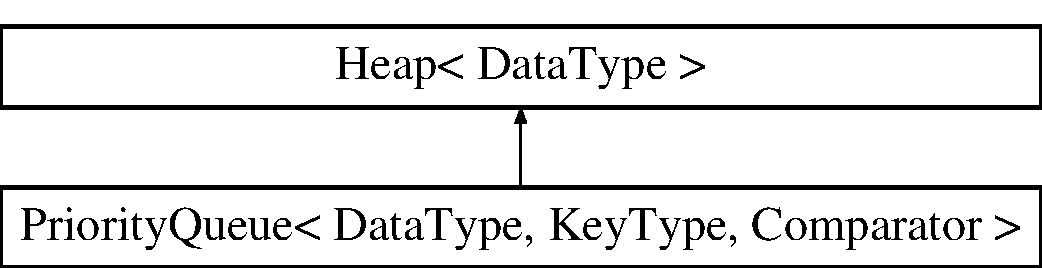
\includegraphics[height=2.000000cm]{class_priority_queue}
\end{center}
\end{figure}
\subsection*{\-Public \-Member \-Functions}
\begin{DoxyCompactItemize}
\item 
\hyperlink{class_priority_queue_a47de2a46cff1d6a6ed30a99c94dc1b14}{\-Priority\-Queue} (int max\-Number=\hyperlink{_priority_queue_8h_a88703212007be018800be64f2f5fde2f}{def\-Max\-Queue\-Size})
\item 
void \hyperlink{class_priority_queue_a61f3339cf0e87c67ed004f8eff0a1bfa}{enqueue} (const \-Data\-Type \&new\-Data\-Item)
\item 
\-Data\-Type \hyperlink{class_priority_queue_a5bc758e313d6244e672ea6e81d695a46}{dequeue} ()
\end{DoxyCompactItemize}
\subsubsection*{template$<$typename Data\-Type, typename Key\-Type = int, typename Comparator = \-Less$<$\-Key\-Type$>$$>$ class Priority\-Queue$<$ Data\-Type, Key\-Type, Comparator $>$}



\subsection{\-Constructor \& \-Destructor \-Documentation}
\hypertarget{class_priority_queue_a47de2a46cff1d6a6ed30a99c94dc1b14}{\index{\-Priority\-Queue@{\-Priority\-Queue}!\-Priority\-Queue@{\-Priority\-Queue}}
\index{\-Priority\-Queue@{\-Priority\-Queue}!PriorityQueue@{\-Priority\-Queue}}
\subsubsection[{\-Priority\-Queue}]{\setlength{\rightskip}{0pt plus 5cm}template$<$typename Data\-Type , typename Key\-Type , typename Comparator $>$ {\bf \-Priority\-Queue}$<$ \-Data\-Type, \-Key\-Type, \-Comparator $>$\-::{\bf \-Priority\-Queue} (
\begin{DoxyParamCaption}
\item[{int}]{max\-Number = {\ttfamily {\bf def\-Max\-Queue\-Size}}}
\end{DoxyParamCaption}
)}}\label{class_priority_queue_a47de2a46cff1d6a6ed30a99c94dc1b14}


\subsection{\-Member \-Function \-Documentation}
\hypertarget{class_priority_queue_a5bc758e313d6244e672ea6e81d695a46}{\index{\-Priority\-Queue@{\-Priority\-Queue}!dequeue@{dequeue}}
\index{dequeue@{dequeue}!PriorityQueue@{\-Priority\-Queue}}
\subsubsection[{dequeue}]{\setlength{\rightskip}{0pt plus 5cm}template$<$typename Data\-Type , typename Key\-Type , typename Comparator $>$ \-Data\-Type {\bf \-Priority\-Queue}$<$ \-Data\-Type, \-Key\-Type, \-Comparator $>$\-::{\bf dequeue} (
\begin{DoxyParamCaption}
{}
\end{DoxyParamCaption}
)}}\label{class_priority_queue_a5bc758e313d6244e672ea6e81d695a46}
\hypertarget{class_priority_queue_a61f3339cf0e87c67ed004f8eff0a1bfa}{\index{\-Priority\-Queue@{\-Priority\-Queue}!enqueue@{enqueue}}
\index{enqueue@{enqueue}!PriorityQueue@{\-Priority\-Queue}}
\subsubsection[{enqueue}]{\setlength{\rightskip}{0pt plus 5cm}template$<$typename Data\-Type , typename Key\-Type , typename Comparator $>$ void {\bf \-Priority\-Queue}$<$ \-Data\-Type, \-Key\-Type, \-Comparator $>$\-::{\bf enqueue} (
\begin{DoxyParamCaption}
\item[{const \-Data\-Type \&}]{new\-Data\-Item}
\end{DoxyParamCaption}
)}}\label{class_priority_queue_a61f3339cf0e87c67ed004f8eff0a1bfa}


\-The documentation for this class was generated from the following files\-:\begin{DoxyCompactItemize}
\item 
\hyperlink{_priority_queue_8h}{\-Priority\-Queue.\-h}\item 
\hyperlink{_priority_queue_8cpp}{\-Priority\-Queue.\-cpp}\end{DoxyCompactItemize}

\hypertarget{struct_task_data}{\section{\-Task\-Data \-Struct \-Reference}
\label{struct_task_data}\index{\-Task\-Data@{\-Task\-Data}}
}
\subsection*{\-Public \-Member \-Functions}
\begin{DoxyCompactItemize}
\item 
int \hyperlink{struct_task_data_a58cbe6eec8a86be7b827561a2f4b49c1}{get\-Priority} () const 
\item 
int \hyperlink{struct_task_data_a58cbe6eec8a86be7b827561a2f4b49c1}{get\-Priority} () const 
\end{DoxyCompactItemize}
\subsection*{\-Public \-Attributes}
\begin{DoxyCompactItemize}
\item 
int \hyperlink{struct_task_data_a9d8b606897eb428a62d816b71312e1b7}{priority}
\item 
int \hyperlink{struct_task_data_a126fafee3369b6a2d8734f4e46c670bc}{arrived}
\end{DoxyCompactItemize}


\subsection{\-Member \-Function \-Documentation}
\hypertarget{struct_task_data_a58cbe6eec8a86be7b827561a2f4b49c1}{\index{\-Task\-Data@{\-Task\-Data}!get\-Priority@{get\-Priority}}
\index{get\-Priority@{get\-Priority}!TaskData@{\-Task\-Data}}
\subsubsection[{get\-Priority}]{\setlength{\rightskip}{0pt plus 5cm}int {\bf \-Task\-Data\-::get\-Priority} (
\begin{DoxyParamCaption}
{}
\end{DoxyParamCaption}
) const\hspace{0.3cm}{\ttfamily  \mbox{[}inline\mbox{]}}}}\label{struct_task_data_a58cbe6eec8a86be7b827561a2f4b49c1}
\hypertarget{struct_task_data_a58cbe6eec8a86be7b827561a2f4b49c1}{\index{\-Task\-Data@{\-Task\-Data}!get\-Priority@{get\-Priority}}
\index{get\-Priority@{get\-Priority}!TaskData@{\-Task\-Data}}
\subsubsection[{get\-Priority}]{\setlength{\rightskip}{0pt plus 5cm}int {\bf \-Task\-Data\-::get\-Priority} (
\begin{DoxyParamCaption}
{}
\end{DoxyParamCaption}
) const\hspace{0.3cm}{\ttfamily  \mbox{[}inline\mbox{]}}}}\label{struct_task_data_a58cbe6eec8a86be7b827561a2f4b49c1}


\subsection{\-Member \-Data \-Documentation}
\hypertarget{struct_task_data_a126fafee3369b6a2d8734f4e46c670bc}{\index{\-Task\-Data@{\-Task\-Data}!arrived@{arrived}}
\index{arrived@{arrived}!TaskData@{\-Task\-Data}}
\subsubsection[{arrived}]{\setlength{\rightskip}{0pt plus 5cm}int {\bf \-Task\-Data\-::arrived}}}\label{struct_task_data_a126fafee3369b6a2d8734f4e46c670bc}
\hypertarget{struct_task_data_a9d8b606897eb428a62d816b71312e1b7}{\index{\-Task\-Data@{\-Task\-Data}!priority@{priority}}
\index{priority@{priority}!TaskData@{\-Task\-Data}}
\subsubsection[{priority}]{\setlength{\rightskip}{0pt plus 5cm}int {\bf \-Task\-Data\-::priority}}}\label{struct_task_data_a9d8b606897eb428a62d816b71312e1b7}


\-The documentation for this struct was generated from the following files\-:\begin{DoxyCompactItemize}
\item 
\hyperlink{ossim_8cpp}{ossim.\-cpp}\item 
\hyperlink{ossim_8cs}{ossim.\-cs}\end{DoxyCompactItemize}

\hypertarget{class_test_data}{\section{\-Test\-Data \-Class \-Reference}
\label{class_test_data}\index{\-Test\-Data@{\-Test\-Data}}
}
\subsection*{\-Public \-Member \-Functions}
\begin{DoxyCompactItemize}
\item 
void \hyperlink{class_test_data_a609b8a4b0e3221bfb0b8cbd9efb108a7}{set\-Key} (int new\-Key)
\item 
int \hyperlink{class_test_data_a85ac27a4361a78d576dd8c10b1f97961}{get\-Key} () const 
\end{DoxyCompactItemize}
\subsection*{\-Private \-Attributes}
\begin{DoxyCompactItemize}
\item 
int \hyperlink{class_test_data_adafb60a315eaa088791c9e40f4a2618f}{key\-Field}
\end{DoxyCompactItemize}


\subsection{\-Member \-Function \-Documentation}
\hypertarget{class_test_data_a85ac27a4361a78d576dd8c10b1f97961}{\index{\-Test\-Data@{\-Test\-Data}!get\-Key@{get\-Key}}
\index{get\-Key@{get\-Key}!TestData@{\-Test\-Data}}
\subsubsection[{get\-Key}]{\setlength{\rightskip}{0pt plus 5cm}int {\bf \-Test\-Data\-::get\-Key} (
\begin{DoxyParamCaption}
{}
\end{DoxyParamCaption}
) const\hspace{0.3cm}{\ttfamily  \mbox{[}inline\mbox{]}}}}\label{class_test_data_a85ac27a4361a78d576dd8c10b1f97961}
\hypertarget{class_test_data_a609b8a4b0e3221bfb0b8cbd9efb108a7}{\index{\-Test\-Data@{\-Test\-Data}!set\-Key@{set\-Key}}
\index{set\-Key@{set\-Key}!TestData@{\-Test\-Data}}
\subsubsection[{set\-Key}]{\setlength{\rightskip}{0pt plus 5cm}void {\bf \-Test\-Data\-::set\-Key} (
\begin{DoxyParamCaption}
\item[{int}]{new\-Key}
\end{DoxyParamCaption}
)\hspace{0.3cm}{\ttfamily  \mbox{[}inline\mbox{]}}}}\label{class_test_data_a609b8a4b0e3221bfb0b8cbd9efb108a7}


\subsection{\-Member \-Data \-Documentation}
\hypertarget{class_test_data_adafb60a315eaa088791c9e40f4a2618f}{\index{\-Test\-Data@{\-Test\-Data}!key\-Field@{key\-Field}}
\index{key\-Field@{key\-Field}!TestData@{\-Test\-Data}}
\subsubsection[{key\-Field}]{\setlength{\rightskip}{0pt plus 5cm}int {\bf \-Test\-Data\-::key\-Field}\hspace{0.3cm}{\ttfamily  \mbox{[}private\mbox{]}}}}\label{class_test_data_adafb60a315eaa088791c9e40f4a2618f}


\-The documentation for this class was generated from the following file\-:\begin{DoxyCompactItemize}
\item 
\hyperlink{test9_8cpp}{test9.\-cpp}\end{DoxyCompactItemize}

\hypertarget{class_test_data_item}{\section{\-Test\-Data\-Item$<$ \-Key\-Type $>$ \-Class \-Template \-Reference}
\label{class_test_data_item}\index{\-Test\-Data\-Item$<$ Key\-Type $>$@{\-Test\-Data\-Item$<$ Key\-Type $>$}}
}
\subsection*{\-Public \-Member \-Functions}
\begin{DoxyCompactItemize}
\item 
\hyperlink{class_test_data_item_adfbd4f5d142caf3d95c96940f96c1d85}{\-Test\-Data\-Item} ()
\item 
void \hyperlink{class_test_data_item_a84667429c081b1dbb212956c88011216}{set\-Priority} (\-Key\-Type new\-Pty)
\item 
\-Key\-Type \hyperlink{class_test_data_item_ac1632213d959555ec8f5aee8a1505d72}{get\-Priority} () const 
\end{DoxyCompactItemize}
\subsection*{\-Private \-Attributes}
\begin{DoxyCompactItemize}
\item 
\-Key\-Type \hyperlink{class_test_data_item_a9b1a2617cb7a831206d189559e8e2e8b}{priority}
\end{DoxyCompactItemize}
\subsubsection*{template$<$typename Key\-Type$>$ class Test\-Data\-Item$<$ Key\-Type $>$}



\subsection{\-Constructor \& \-Destructor \-Documentation}
\hypertarget{class_test_data_item_adfbd4f5d142caf3d95c96940f96c1d85}{\index{\-Test\-Data\-Item@{\-Test\-Data\-Item}!\-Test\-Data\-Item@{\-Test\-Data\-Item}}
\index{\-Test\-Data\-Item@{\-Test\-Data\-Item}!TestDataItem@{\-Test\-Data\-Item}}
\subsubsection[{\-Test\-Data\-Item}]{\setlength{\rightskip}{0pt plus 5cm}template$<$typename Key\-Type $>$ {\bf \-Test\-Data\-Item}$<$ \-Key\-Type $>$\-::{\bf \-Test\-Data\-Item} (
\begin{DoxyParamCaption}
{}
\end{DoxyParamCaption}
)\hspace{0.3cm}{\ttfamily  \mbox{[}inline\mbox{]}}}}\label{class_test_data_item_adfbd4f5d142caf3d95c96940f96c1d85}


\subsection{\-Member \-Function \-Documentation}
\hypertarget{class_test_data_item_ac1632213d959555ec8f5aee8a1505d72}{\index{\-Test\-Data\-Item@{\-Test\-Data\-Item}!get\-Priority@{get\-Priority}}
\index{get\-Priority@{get\-Priority}!TestDataItem@{\-Test\-Data\-Item}}
\subsubsection[{get\-Priority}]{\setlength{\rightskip}{0pt plus 5cm}template$<$typename Key\-Type $>$ \-Key\-Type {\bf \-Test\-Data\-Item}$<$ \-Key\-Type $>$\-::{\bf get\-Priority} (
\begin{DoxyParamCaption}
{}
\end{DoxyParamCaption}
) const\hspace{0.3cm}{\ttfamily  \mbox{[}inline\mbox{]}}}}\label{class_test_data_item_ac1632213d959555ec8f5aee8a1505d72}
\hypertarget{class_test_data_item_a84667429c081b1dbb212956c88011216}{\index{\-Test\-Data\-Item@{\-Test\-Data\-Item}!set\-Priority@{set\-Priority}}
\index{set\-Priority@{set\-Priority}!TestDataItem@{\-Test\-Data\-Item}}
\subsubsection[{set\-Priority}]{\setlength{\rightskip}{0pt plus 5cm}template$<$typename Key\-Type $>$ void {\bf \-Test\-Data\-Item}$<$ \-Key\-Type $>$\-::{\bf set\-Priority} (
\begin{DoxyParamCaption}
\item[{\-Key\-Type}]{new\-Pty}
\end{DoxyParamCaption}
)\hspace{0.3cm}{\ttfamily  \mbox{[}inline\mbox{]}}}}\label{class_test_data_item_a84667429c081b1dbb212956c88011216}


\subsection{\-Member \-Data \-Documentation}
\hypertarget{class_test_data_item_a9b1a2617cb7a831206d189559e8e2e8b}{\index{\-Test\-Data\-Item@{\-Test\-Data\-Item}!priority@{priority}}
\index{priority@{priority}!TestDataItem@{\-Test\-Data\-Item}}
\subsubsection[{priority}]{\setlength{\rightskip}{0pt plus 5cm}template$<$typename Key\-Type $>$ \-Key\-Type {\bf \-Test\-Data\-Item}$<$ \-Key\-Type $>$\-::{\bf priority}\hspace{0.3cm}{\ttfamily  \mbox{[}private\mbox{]}}}}\label{class_test_data_item_a9b1a2617cb7a831206d189559e8e2e8b}


\-The documentation for this class was generated from the following file\-:\begin{DoxyCompactItemize}
\item 
\hyperlink{test11_8cpp}{test11.\-cpp}\end{DoxyCompactItemize}

\chapter{\-File \-Documentation}
\hypertarget{config_8h}{\section{config.\-h \-File \-Reference}
\label{config_8h}\index{config.\-h@{config.\-h}}
}
\subsection*{\-Defines}
\begin{DoxyCompactItemize}
\item 
\#define \hyperlink{config_8h_a350537e3c8a46e223080118d09ef0b10}{\-L\-A\-B11\-\_\-\-T\-E\-S\-T1}~1
\end{DoxyCompactItemize}


\subsection{\-Define \-Documentation}
\hypertarget{config_8h_a350537e3c8a46e223080118d09ef0b10}{\index{config.\-h@{config.\-h}!\-L\-A\-B11\-\_\-\-T\-E\-S\-T1@{\-L\-A\-B11\-\_\-\-T\-E\-S\-T1}}
\index{\-L\-A\-B11\-\_\-\-T\-E\-S\-T1@{\-L\-A\-B11\-\_\-\-T\-E\-S\-T1}!config.h@{config.\-h}}
\subsubsection[{\-L\-A\-B11\-\_\-\-T\-E\-S\-T1}]{\setlength{\rightskip}{0pt plus 5cm}\#define {\bf \-L\-A\-B11\-\_\-\-T\-E\-S\-T1}~1}}\label{config_8h_a350537e3c8a46e223080118d09ef0b10}
\hyperlink{class_heap}{\-Heap} class configuration file. \-Activate test \#\-N by defining the corresponding \-L\-A\-B11\-\_\-\-T\-E\-S\-T\-N to have the value 1. 
\hypertarget{_heap_8cpp}{\section{\-Heap.\-cpp \-File \-Reference}
\label{_heap_8cpp}\index{\-Heap.\-cpp@{\-Heap.\-cpp}}
}
{\ttfamily \#include \char`\"{}\-Heap.\-h\char`\"{}}\*

\hypertarget{_heap_8h}{\section{\-Heap.\-h \-File \-Reference}
\label{_heap_8h}\index{\-Heap.\-h@{\-Heap.\-h}}
}
{\ttfamily \#include $<$stdexcept$>$}\*
{\ttfamily \#include $<$iostream$>$}\*
\subsection*{\-Classes}
\begin{DoxyCompactItemize}
\item 
class \hyperlink{class_less}{\-Less$<$ Key\-Type $>$}
\item 
class \hyperlink{class_heap}{\-Heap$<$ Data\-Type, Key\-Type, Comparator $>$}
\end{DoxyCompactItemize}

\hypertarget{heapsort_8cs}{\section{heapsort.\-cs \-File \-Reference}
\label{heapsort_8cs}\index{heapsort.\-cs@{heapsort.\-cs}}
}
\subsection*{\-Functions}
\begin{DoxyCompactItemize}
\item 
{\footnotesize template$<$typename Data\-Type $>$ }\\void \hyperlink{heapsort_8cs_ace0c151b0a221e24a1aad0bf9a821c2f}{move\-Down} (\-Data\-Type data\-Items\mbox{[}$\,$\mbox{]}, int root, int size)
\item 
{\footnotesize template$<$typename Data\-Type $>$ }\\void \hyperlink{heapsort_8cs_a1b9d07732ab0ab5fb1c3fabfb8ba4f4b}{heap\-Sort} (\-Data\-Type data\-Items\mbox{[}$\,$\mbox{]}, int size)
\end{DoxyCompactItemize}


\subsection{\-Function \-Documentation}
\hypertarget{heapsort_8cs_a1b9d07732ab0ab5fb1c3fabfb8ba4f4b}{\index{heapsort.\-cs@{heapsort.\-cs}!heap\-Sort@{heap\-Sort}}
\index{heap\-Sort@{heap\-Sort}!heapsort.cs@{heapsort.\-cs}}
\subsubsection[{heap\-Sort}]{\setlength{\rightskip}{0pt plus 5cm}template$<$typename Data\-Type $>$ void {\bf heap\-Sort} (
\begin{DoxyParamCaption}
\item[{\-Data\-Type}]{data\-Items\mbox{[}$\,$\mbox{]}, }
\item[{int}]{size}
\end{DoxyParamCaption}
)}}\label{heapsort_8cs_a1b9d07732ab0ab5fb1c3fabfb8ba4f4b}
\hypertarget{heapsort_8cs_ace0c151b0a221e24a1aad0bf9a821c2f}{\index{heapsort.\-cs@{heapsort.\-cs}!move\-Down@{move\-Down}}
\index{move\-Down@{move\-Down}!heapsort.cs@{heapsort.\-cs}}
\subsubsection[{move\-Down}]{\setlength{\rightskip}{0pt plus 5cm}template$<$typename Data\-Type $>$ void {\bf move\-Down} (
\begin{DoxyParamCaption}
\item[{\-Data\-Type}]{data\-Items\mbox{[}$\,$\mbox{]}, }
\item[{int}]{root, }
\item[{int}]{size}
\end{DoxyParamCaption}
)}}\label{heapsort_8cs_ace0c151b0a221e24a1aad0bf9a821c2f}

\hypertarget{ossim_8cpp}{\section{ossim.\-cpp \-File \-Reference}
\label{ossim_8cpp}\index{ossim.\-cpp@{ossim.\-cpp}}
}
{\ttfamily \#include $<$iostream$>$}\*
{\ttfamily \#include $<$cstdlib$>$}\*
{\ttfamily \#include \char`\"{}\-Priority\-Queue.\-cpp\char`\"{}}\*
\subsection*{\-Classes}
\begin{DoxyCompactItemize}
\item 
struct \hyperlink{struct_task_data}{\-Task\-Data}
\end{DoxyCompactItemize}
\subsection*{\-Functions}
\begin{DoxyCompactItemize}
\item 
int \hyperlink{ossim_8cpp_ae66f6b31b5ad750f1fe042a706a4e3d4}{main} ()
\end{DoxyCompactItemize}


\subsection{\-Function \-Documentation}
\hypertarget{ossim_8cpp_ae66f6b31b5ad750f1fe042a706a4e3d4}{\index{ossim.\-cpp@{ossim.\-cpp}!main@{main}}
\index{main@{main}!ossim.cpp@{ossim.\-cpp}}
\subsubsection[{main}]{\setlength{\rightskip}{0pt plus 5cm}int {\bf main} (
\begin{DoxyParamCaption}
{}
\end{DoxyParamCaption}
)}}\label{ossim_8cpp_ae66f6b31b5ad750f1fe042a706a4e3d4}

\hypertarget{ossim_8cs}{\section{ossim.\-cs \-File \-Reference}
\label{ossim_8cs}\index{ossim.\-cs@{ossim.\-cs}}
}
{\ttfamily \#include $<$iostream$>$}\*
{\ttfamily \#include $<$cstdlib$>$}\*
{\ttfamily \#include \char`\"{}\-Priority\-Queue.\-cpp\char`\"{}}\*
\subsection*{\-Classes}
\begin{DoxyCompactItemize}
\item 
struct \hyperlink{struct_task_data}{\-Task\-Data}
\end{DoxyCompactItemize}
\subsection*{\-Functions}
\begin{DoxyCompactItemize}
\item 
int \hyperlink{ossim_8cs_ae66f6b31b5ad750f1fe042a706a4e3d4}{main} ()
\end{DoxyCompactItemize}


\subsection{\-Function \-Documentation}
\hypertarget{ossim_8cs_ae66f6b31b5ad750f1fe042a706a4e3d4}{\index{ossim.\-cs@{ossim.\-cs}!main@{main}}
\index{main@{main}!ossim.cs@{ossim.\-cs}}
\subsubsection[{main}]{\setlength{\rightskip}{0pt plus 5cm}int {\bf main} (
\begin{DoxyParamCaption}
{}
\end{DoxyParamCaption}
)}}\label{ossim_8cs_ae66f6b31b5ad750f1fe042a706a4e3d4}

\hypertarget{_priority_queue_8cpp}{\section{\-Priority\-Queue.\-cpp \-File \-Reference}
\label{_priority_queue_8cpp}\index{\-Priority\-Queue.\-cpp@{\-Priority\-Queue.\-cpp}}
}
{\ttfamily \#include \char`\"{}\-Priority\-Queue.\-h\char`\"{}}\*

\hypertarget{_priority_queue_8h}{\section{\-Priority\-Queue.\-h \-File \-Reference}
\label{_priority_queue_8h}\index{\-Priority\-Queue.\-h@{\-Priority\-Queue.\-h}}
}
{\ttfamily \#include $<$stdexcept$>$}\*
{\ttfamily \#include $<$iostream$>$}\*
{\ttfamily \#include \char`\"{}\-Heap.\-cpp\char`\"{}}\*
\subsection*{\-Classes}
\begin{DoxyCompactItemize}
\item 
class \hyperlink{class_priority_queue}{\-Priority\-Queue$<$ Data\-Type, Key\-Type, Comparator $>$}
\end{DoxyCompactItemize}
\subsection*{\-Variables}
\begin{DoxyCompactItemize}
\item 
const int \hyperlink{_priority_queue_8h_a88703212007be018800be64f2f5fde2f}{def\-Max\-Queue\-Size} = 10
\end{DoxyCompactItemize}


\subsection{\-Variable \-Documentation}
\hypertarget{_priority_queue_8h_a88703212007be018800be64f2f5fde2f}{\index{\-Priority\-Queue.\-h@{\-Priority\-Queue.\-h}!def\-Max\-Queue\-Size@{def\-Max\-Queue\-Size}}
\index{def\-Max\-Queue\-Size@{def\-Max\-Queue\-Size}!PriorityQueue.h@{\-Priority\-Queue.\-h}}
\subsubsection[{def\-Max\-Queue\-Size}]{\setlength{\rightskip}{0pt plus 5cm}const int {\bf def\-Max\-Queue\-Size} = 10}}\label{_priority_queue_8h_a88703212007be018800be64f2f5fde2f}

\hypertarget{show11_8cpp}{\section{show11.\-cpp \-File \-Reference}
\label{show11_8cpp}\index{show11.\-cpp@{show11.\-cpp}}
}

\hypertarget{test11_8cpp}{\section{test11.\-cpp \-File \-Reference}
\label{test11_8cpp}\index{test11.\-cpp@{test11.\-cpp}}
}
{\ttfamily \#include $<$iostream$>$}\*
{\ttfamily \#include $<$string$>$}\*
{\ttfamily \#include $<$cctype$>$}\*
{\ttfamily \#include \char`\"{}\-Heap.\-cpp\char`\"{}}\*
{\ttfamily \#include \char`\"{}config.\-h\char`\"{}}\*
\subsection*{\-Classes}
\begin{DoxyCompactItemize}
\item 
class \hyperlink{class_test_data_item}{\-Test\-Data\-Item$<$ Key\-Type $>$}
\item 
class \hyperlink{class_greater}{\-Greater$<$ Key\-Type $>$}
\end{DoxyCompactItemize}
\subsection*{\-Functions}
\begin{DoxyCompactItemize}
\item 
void \hyperlink{test11_8cpp_a0d20b69b0ad703df78459e1033d5c1d4}{print\-Help} ()
\item 
int \hyperlink{test11_8cpp_ae66f6b31b5ad750f1fe042a706a4e3d4}{main} ()
\end{DoxyCompactItemize}


\subsection{\-Function \-Documentation}
\hypertarget{test11_8cpp_ae66f6b31b5ad750f1fe042a706a4e3d4}{\index{test11.\-cpp@{test11.\-cpp}!main@{main}}
\index{main@{main}!test11.cpp@{test11.\-cpp}}
\subsubsection[{main}]{\setlength{\rightskip}{0pt plus 5cm}int {\bf main} (
\begin{DoxyParamCaption}
{}
\end{DoxyParamCaption}
)}}\label{test11_8cpp_ae66f6b31b5ad750f1fe042a706a4e3d4}
\hypertarget{test11_8cpp_a0d20b69b0ad703df78459e1033d5c1d4}{\index{test11.\-cpp@{test11.\-cpp}!print\-Help@{print\-Help}}
\index{print\-Help@{print\-Help}!test11.cpp@{test11.\-cpp}}
\subsubsection[{print\-Help}]{\setlength{\rightskip}{0pt plus 5cm}void {\bf print\-Help} (
\begin{DoxyParamCaption}
{}
\end{DoxyParamCaption}
)}}\label{test11_8cpp_a0d20b69b0ad703df78459e1033d5c1d4}

\hypertarget{test11hs_8cpp}{\section{test11hs.\-cpp \-File \-Reference}
\label{test11hs_8cpp}\index{test11hs.\-cpp@{test11hs.\-cpp}}
}
{\ttfamily \#include $<$iostream$>$}\*
{\ttfamily \#include \char`\"{}heapsort.\-cpp\char`\"{}}\*
\subsection*{\-Classes}
\begin{DoxyCompactItemize}
\item 
class \hyperlink{class_test_data}{\-Test\-Data}
\end{DoxyCompactItemize}
\subsection*{\-Functions}
\begin{DoxyCompactItemize}
\item 
int \hyperlink{test11hs_8cpp_ae66f6b31b5ad750f1fe042a706a4e3d4}{main} ()
\end{DoxyCompactItemize}
\subsection*{\-Variables}
\begin{DoxyCompactItemize}
\item 
const int \hyperlink{test11hs_8cpp_af9ecea2a656a85cc42eb181a9976ad31}{\-M\-A\-X\-\_\-\-N\-U\-M\-\_\-\-D\-A\-T\-A\-\_\-\-I\-T\-E\-M\-S} = 10
\end{DoxyCompactItemize}


\subsection{\-Function \-Documentation}
\hypertarget{test11hs_8cpp_ae66f6b31b5ad750f1fe042a706a4e3d4}{\index{test11hs.\-cpp@{test11hs.\-cpp}!main@{main}}
\index{main@{main}!test11hs.cpp@{test11hs.\-cpp}}
\subsubsection[{main}]{\setlength{\rightskip}{0pt plus 5cm}int {\bf main} (
\begin{DoxyParamCaption}
{}
\end{DoxyParamCaption}
)}}\label{test11hs_8cpp_ae66f6b31b5ad750f1fe042a706a4e3d4}


\subsection{\-Variable \-Documentation}
\hypertarget{test11hs_8cpp_af9ecea2a656a85cc42eb181a9976ad31}{\index{test11hs.\-cpp@{test11hs.\-cpp}!\-M\-A\-X\-\_\-\-N\-U\-M\-\_\-\-D\-A\-T\-A\-\_\-\-I\-T\-E\-M\-S@{\-M\-A\-X\-\_\-\-N\-U\-M\-\_\-\-D\-A\-T\-A\-\_\-\-I\-T\-E\-M\-S}}
\index{\-M\-A\-X\-\_\-\-N\-U\-M\-\_\-\-D\-A\-T\-A\-\_\-\-I\-T\-E\-M\-S@{\-M\-A\-X\-\_\-\-N\-U\-M\-\_\-\-D\-A\-T\-A\-\_\-\-I\-T\-E\-M\-S}!test11hs.cpp@{test11hs.\-cpp}}
\subsubsection[{\-M\-A\-X\-\_\-\-N\-U\-M\-\_\-\-D\-A\-T\-A\-\_\-\-I\-T\-E\-M\-S}]{\setlength{\rightskip}{0pt plus 5cm}const int {\bf \-M\-A\-X\-\_\-\-N\-U\-M\-\_\-\-D\-A\-T\-A\-\_\-\-I\-T\-E\-M\-S} = 10}}\label{test11hs_8cpp_af9ecea2a656a85cc42eb181a9976ad31}

\hypertarget{test11pq_8cpp}{\section{test11pq.\-cpp \-File \-Reference}
\label{test11pq_8cpp}\index{test11pq.\-cpp@{test11pq.\-cpp}}
}
{\ttfamily \#include $<$iostream$>$}\*
{\ttfamily \#include $<$cctype$>$}\*
{\ttfamily \#include \char`\"{}\-Priority\-Queue.\-cpp\char`\"{}}\*
\subsection*{\-Classes}
\begin{DoxyCompactItemize}
\item 
class \hyperlink{class_test_data}{\-Test\-Data}
\end{DoxyCompactItemize}
\subsection*{\-Functions}
\begin{DoxyCompactItemize}
\item 
void \hyperlink{test11pq_8cpp_a0d20b69b0ad703df78459e1033d5c1d4}{print\-Help} ()
\item 
int \hyperlink{test11pq_8cpp_ae66f6b31b5ad750f1fe042a706a4e3d4}{main} ()
\end{DoxyCompactItemize}


\subsection{\-Function \-Documentation}
\hypertarget{test11pq_8cpp_ae66f6b31b5ad750f1fe042a706a4e3d4}{\index{test11pq.\-cpp@{test11pq.\-cpp}!main@{main}}
\index{main@{main}!test11pq.cpp@{test11pq.\-cpp}}
\subsubsection[{main}]{\setlength{\rightskip}{0pt plus 5cm}int {\bf main} (
\begin{DoxyParamCaption}
{}
\end{DoxyParamCaption}
)}}\label{test11pq_8cpp_ae66f6b31b5ad750f1fe042a706a4e3d4}
\hypertarget{test11pq_8cpp_a0d20b69b0ad703df78459e1033d5c1d4}{\index{test11pq.\-cpp@{test11pq.\-cpp}!print\-Help@{print\-Help}}
\index{print\-Help@{print\-Help}!test11pq.cpp@{test11pq.\-cpp}}
\subsubsection[{print\-Help}]{\setlength{\rightskip}{0pt plus 5cm}void {\bf print\-Help} (
\begin{DoxyParamCaption}
{}
\end{DoxyParamCaption}
)}}\label{test11pq_8cpp_a0d20b69b0ad703df78459e1033d5c1d4}

\printindex
\end{document}
